\documentclass[11pt]{amsart}
\usepackage[a4paper,margin=28mm]{geometry}
\usepackage{amsmath,amssymb,amsthm,graphicx,booktabs,hyperref,enumitem}

\newtheorem{theorem}{Theorem}
\newtheorem{proposition}{Proposition}[section]
\newtheorem{lemma}[proposition]{Lemma}
\theoremstyle{remark}
\newtheorem{remark}[proposition]{Remark}

\newcommand{\U}{\mathcal U}
\newcommand{\D}{\mathbb D}
\newcommand{\C}{\mathbb C}
\newcommand{\Z}{\mathbb Z}
\newcommand{\re}{\operatorname{Re}}
\newcommand{\im}{\operatorname{Im}}
\newcommand{\dist}{\operatorname{dist}}
\newcommand{\dmu}{\frac{dy}{\sqrt{1-y^2}}}

\hypersetup{pdftitle={An improved upper bound for the univalent Bloch-Landau constant},pdfauthor={Wynand van Staden}}
\title[The univalent Bloch--Landau constant]{An improved upper bound for the univalent Bloch--Landau constant}
\author{Wynand van Staden}
\date{Draft of 13 October 2026. Not submitted. Prepared with substantial AI assistance; see Section~\ref{sec:disclosure}.}

\begin{document}

\begin{abstract}
We exhibit a disc with $24$ slits, $18$ of them curved, for which the ratio of inradius to conformal radius
is less than $0.65628589$. This improves the best proved upper bound $0.6563937$ for the univalent
Bloch--Landau constant (Carroll and Ortega-Cerd\`a, 2009) and lies below the best numerical value
$0.656319277$ in the literature (Ortega-Cerd\`a and Pridhnani, 2010). The bound is established by a
computer-assisted proof: the inradius is bounded by an exact covering argument, and the conformal radius is
bounded below by a comparison function whose boundary values are controlled in ball arithmetic.
The domain was found by an evolutionary search driven by a spectral integral-equation solver.
\end{abstract}

\maketitle

\section{Introduction}

Let $\D$ be the unit disc. The \emph{univalent Bloch--Landau constant} $\U$ is the largest number such that
$f(\D)$ contains a disc of radius $\U$ for every univalent $f$ on $\D$ with $|f'(0)|=1$.
For a domain $D\subset\C$ write $R(D)$ for its \emph{inradius}, the supremum of the radii of the discs contained
in $D$. If $D\ne\C$ is simply connected and $0\in D$, write $\rho(D)$ for its \emph{conformal radius} at $0$,
that is $|f'(0)|$ for a conformal map $f$ of $\D$ onto $D$ with $f(0)=0$. Applying the definition to $f/f'(0)$,
\begin{equation}\label{eq:basic}
\U\le\frac{R(D)}{\rho(D)}\qquad\text{for every simply connected }D\ne\C\text{ with }0\in D,
\end{equation}
and $\U$ is the infimum of the right-hand side. Every upper bound for $\U$ so far has been obtained from
\eqref{eq:basic} with $D$ a disc from which slits have been removed (Table~\ref{tab:history}).

\begin{table}[h]
\centering\small
\begin{tabular}{llll}
\toprule
 & upper bound & domain & nature\\
\midrule
Robinson \cite{Rob} (1935) & $0.658$ & six radial slits & closed form\\
Goodman \cite{Good} (1945) & $0.65647$ & generations of radial slits & closed form\\
Beller, Hummel \cite{BH} (1985) & $0.6564155$ & twelve radial slits & numerical\\
Carroll, Ortega-Cerd\`a \cite{COC} (2009) & $0.6563937$ & radial slits and forked arcs & closed form\\
Ortega-Cerd\`a, Pridhnani \cite{OCP} (2010) & $0.656319277$ & two forked arcs per half-sector & numerical\\
\bottomrule
\end{tabular}
\caption{Upper bounds for $\U$. The authors of \cite{OCP} state that no rigorous error analysis was made for
their value. The best lower bound known to us is $0.5708858$ \cite{Sk}.}\label{tab:history}
\end{table}

\begin{theorem}\label{thm:main}
$\U<0.65628589$.
\end{theorem}

The domain $D$ that proves Theorem~\ref{thm:main} is described in Section~\ref{sec:domain}. The proof has two
independent parts:
\[
R(D)\le 1+10^{-9}\quad\text{(Proposition \ref{prop:inradius})},\qquad
\rho(D)\ge 1.523726208329\quad\text{(Proposition \ref{prop:rho})},
\]
and $(1+10^{-9})/1.523726208329<0.65628589$.
Both parts rely on computations, carried out in exact integer arithmetic or in ball arithmetic with the Arb
library \cite{Arb}; the programs are part of the repository accompanying this paper and run in about one minute.
Section~\ref{sec:numerics} describes how the domain was found and the independent numerical checks, none of
which is used in the proof.

The domains of \cite{COC,OCP} satisfy a necessary condition for extremality (harmonic symmetry of the free arcs)
which makes them amenable to explicit formulas. No such condition is imposed here: the slits are taken from a
four-parameter family and optimised numerically. The resulting domain nevertheless resembles the tree-like domains
of \cite{COC,OCP} (Figure~\ref{fig:domain}).

\section{The domain}\label{sec:domain}

Fix $R>0$. A \emph{slit} with parameters $(\theta,t,b_1,b_2)$, $0<t<R$, is the arc
\begin{equation}\label{eq:slit}
z=\exp w(x),\qquad w(x)=L+ax+i\bigl(\theta+b_1(ax)^2+b_2(ax)^4\bigr),\qquad -1\le x\le0,
\end{equation}
where $L=\log R$ and $a=\log(R/t)>0$. Since $|z|=Re^{ax}$, the slit starts on the circle $|z|=R$ at $Re^{i\theta}$,
its modulus decreases monotonically along it, and it ends at a tip of modulus $t$. For $b_1=b_2=0$ it is the radial
segment $[te^{i\theta},Re^{i\theta}]$.

Let $R=5.001117628756668$. The slits of our domain are those with the parameters $(\theta,t,b_1,b_2)$ of
Table~\ref{tab:params} together with their images under the group generated by $z\mapsto e^{2\pi i/3}z$ and
$z\mapsto\bar z$, that is, the slits with parameters $(2\pi r/3\pm\theta,\,t,\,\pm b_1,\,\pm b_2)$, $r=0,1,2$.
This gives $24$ slits in five classes. All decimal numbers in this section are to be read as exact rational numbers.

\begin{table}[h]
\centering\footnotesize\setlength{\tabcolsep}{4pt}
\begin{tabular}{clllll}
\toprule
class & $\theta$ & $t$ & $b_1$ & $b_2$ & slits\\
\midrule
0 & $0$ & $1$ & $0$ & $0$ & 3\\
1 & $\pi/3$ & $1.9999999974092333$ & $0$ & $0$ & 3\\
2 & $0.029930188727091613$ & $2.789342409403121$ & $0.9026921410641155$ & $-0.3301459494660587$ & 6\\
3 & $1.0157094972537686$ & $3.473381248030611$ & $-1.2656124700253997$ & $0.9794269477754911$ & 6\\
4 & $0.5757776442359243$ & $4.342874184977691$ & $0.03225521024585182$ & $2.9360081049550737$ & 6\\
\bottomrule
\end{tabular}
\caption{The parameters of the domain; $R=5.001117628756668$.}\label{tab:params}
\end{table}

Let $K$ be the union of the $24$ slits and let $D$ be the connected component of
$\{|z|<R\}\setminus K$ that contains $0$.

\begin{lemma}\label{lem:sc}
$D$ is a simply connected domain, $0\in D\ne\C$, and $\partial D\subset\{|z|=R\}\cup K$. In particular
\eqref{eq:basic} applies to $D$.
\end{lemma}

\begin{proof}
Every point of $K$ has modulus at least $1$, so $0\notin K$. Each slit is connected and meets the circle
$|z|=R$, so $E=\{|z|\ge R\}\cup\{\infty\}\cup K$ is a closed connected subset of the Riemann sphere. Every
component of the complement of a closed connected subset of the sphere is simply connected, and $D$ is such a
component. The statement about the boundary is clear.
\end{proof}

\begin{remark}
The slits are in fact pairwise disjoint (the smallest distance between two of them is about $0.1484$), so
$D=\{|z|<R\}\setminus K$; this is not needed for the proof.
\end{remark}

\begin{figure}[h]
\centering
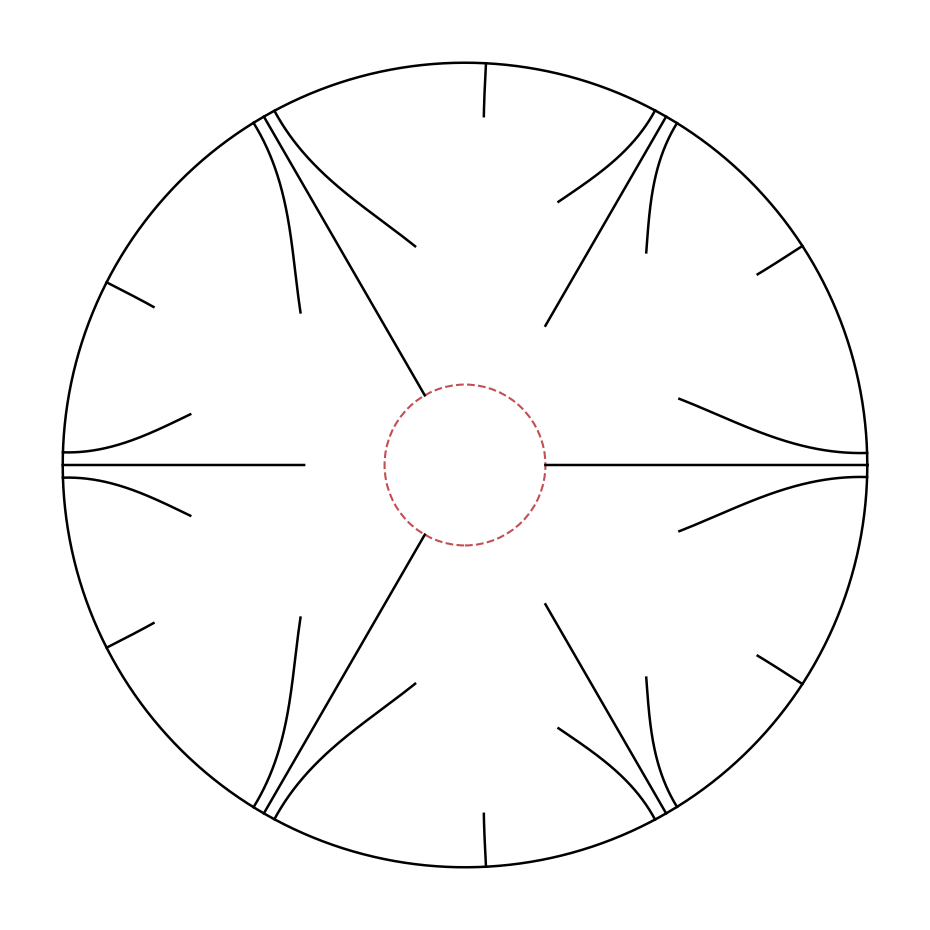
\includegraphics[width=0.62\textwidth]{../domain_G.png}
\caption{The domain $D$. The disc $|z|<1$ is one of $22$ discs of radius between $1-4\times10^{-6}$ and $1$
that are locally largest.}\label{fig:domain}
\end{figure}

\section{The inradius}\label{sec:inradius}

\begin{proposition}\label{prop:inradius}
$R(D)\le1+10^{-9}$.
\end{proposition}

The proof rests on two elementary observations.

\begin{lemma}\label{lem:witness}
If the disc of centre $p$ and radius $r$ is contained in $D$ and $q\notin D$, then $r\le|p-q|$.
\end{lemma}

\begin{lemma}\label{lem:cell}
Let $C$ be a closed square, $q\in\C$ and $\lambda>0$. If $|p-q|\le\lambda$ at the four corners $p$ of $C$,
then $|p-q|\le\lambda$ for all $p\in C$.
\end{lemma}

\begin{proof}
$p\mapsto|p-q|$ is convex, and $C$ is the convex hull of its corners.
\end{proof}

\begin{proof}[Proof of Proposition \ref{prop:inradius}]
Put $\lambda=1+10^{-9}$. The domain is invariant under $z\mapsto e^{2\pi i/3}z$ and $z\mapsto\bar z$,
so it suffices to show that no disc of radius greater than $\lambda$ contained in $D$ has its centre in
$S=\{p:\ 0\le\arg p\le\pi/3,\ |p|<R\}\cup\{0\}$. Note $S\subset[0,8]^2$.

The program \texttt{inradius\_certificate.py} produces a finite family of closed squares (\emph{cells}) of the form
$[i2^{3-\ell},(i+1)2^{3-\ell}]\times[j2^{3-\ell},(j+1)2^{3-\ell}]$ with integers $\ell\ge6$ and
$0\le i,j<2^\ell$, and verifies the following.
\begin{enumerate}[label=(\roman*),leftmargin=2.2em]
\item \emph{The cells cover $[0,8]^2$.} No cell is contained in another, and the areas of the cells add up to $64$;
both statements are checked in exact arithmetic. Since two dyadic squares are either nested or have disjoint
interiors, the cells tile the square.
\item Each cell $[x_0,x_1]\times[y_0,y_1]$ is of one of three kinds:
\begin{itemize}[leftmargin=1.5em]
\item[(a)] $x_0^2+y_0^2\ge R^2$. Then the cell does not meet the open disc $|p|<R$.
\item[(b)] $y_0^2>3x_1^2$. Then every point of the cell has $\arg p>\pi/3$, so the cell does not meet $S$.
\item[(c)] A point $q\notin D$ is specified with $|p-q|\le\lambda$ at the four corners of the cell. By
Lemmas \ref{lem:cell} and \ref{lem:witness}, no disc of radius greater than $\lambda$ contained in $D$ has its
centre in the cell.
\end{itemize}
\end{enumerate}
In (c) the point $q$ is a point $\exp w(x)$ of one of the slits \eqref{eq:slit}, with $x\in[-1,0]$, or a point of
the circle $|z|=R$; such points do not belong to $D$. For a slit point the parameter is given as a
double-precision number $s=ax$ (an exact rational), and $-a<s\le0$ is verified in ball arithmetic, or it is the
tip $s=-a$. The coordinates of $q$ are enclosed in ball arithmetic and replaced by a dyadic rational point $q'$
with $|q-q'|<2^{-69}$; the inequality actually checked, in exact integer arithmetic, is
$|p-q'|^2\le(\lambda-2^{-69})^2$ at the four corners. The inequalities in (a) and (b) involve only rational numbers and are checked exactly.

The run for the domain of Section~\ref{sec:domain} produces $4993$ cells: $2799$ of kind (a), $464$ of kind (b)
and $1730$ of kind (c), the latter using $610$ distinct points $q$. The smallest cells have side $2^{-29}$.
\end{proof}

The cells and the points $q$ are found by a floating-point search which plays no role in the proof: only its
output is verified.

\section{The conformal radius}\label{sec:rho}

\begin{proposition}\label{prop:rho}
$\rho(D)\ge1.523726208329$.
\end{proposition}

\subsection{The comparison principle}

\begin{lemma}\label{lem:comparison}
Let $v$ be continuous on $\overline D\setminus\{0\}$, harmonic in $D\setminus\{0\}$, with
$v(z)=-\log|z|+c+o(1)$ as $z\to0$ and $v\le0$ on $\partial D$. Then $\log\rho(D)\ge c$.
\end{lemma}

\begin{proof}
Let $\varphi$ map $D$ conformally onto $\D$ with $\varphi(0)=0$, and $g=-\log|\varphi|$. Then $g>0$ is harmonic in
$D\setminus\{0\}$ and $g(z)=-\log|z|+\log\rho(D)+o(1)$ at $0$, because $\varphi(z)=z/(\rho(D)e^{i\gamma})+O(z^2)$.
The function $g-v$ is harmonic in $D\setminus\{0\}$ and bounded near $0$, hence harmonic in $D$. At every boundary
point $\liminf(g-v)\ge-\limsup v\ge0$, since $g>0$ and $v$ is continuous with $v\le0$ on $\partial D$. By the
minimum principle $g-v\ge0$ in $D$, and its value at $0$ is $\log\rho(D)-c$.
\end{proof}

\subsection{The comparison function}\label{sec:U}

We work in the variable $w=\log z$ and use the notation of \eqref{eq:slit}, with a subscript $j$ for the $j$-th
slit. We extend $w_j$ to $-1\le x\le1$ by the same formula and call $\Gamma_j=w_j([-1,1])$ an \emph{arc}; the slit
is $w_j([-1,0])$ and the rest, $w_j((0,1])$, lies in the half-plane $\re w>L$. The reflection
$\sigma(w)=2L-\bar w$ in the line $\re w=L$ satisfies
\begin{equation}\label{eq:sigma}
\sigma(w_j(x))=w_j(-x),
\end{equation}
because the imaginary part of $w_j$ is even in $x$. Put
\[
\Phi(w)=-\log\bigl|2\sinh(w/2)\bigr| .
\]
$\Phi$ is harmonic in $\C\setminus2\pi i\Z$, it is $2\pi i$-periodic, $\Phi(-w)=\Phi(\bar w)=\Phi(w)$, and
\begin{equation}\label{eq:phi-asym}
\Phi(w)=-\tfrac12|\re w|-\log\bigl|1-e^{-|\re w|-i\,\im w\,\mathrm{sgn}(\re w)}\bigr|=-\tfrac12|\re w|+O(e^{-|\re w|}).
\end{equation}

For each slit let $\psi_j$ be a real polynomial that is \emph{odd}, with Chebyshev expansion
$\psi_j=\sum_{n\ \mathrm{odd}}c_{j,n}T_n$, and assume that $\psi_j=\psi_{j'}$ whenever the slits $j$ and $j'$
belong to the same class. Define
\begin{equation}\label{eq:U}
U(w)=(L-\re w)+\sum_j\int_{-1}^{1}\Phi\bigl(w-w_j(y)\bigr)\,\psi_j(y)\,\dmu .
\end{equation}

\begin{lemma}\label{lem:U}
\begin{enumerate}[label=(\alph*),leftmargin=2.2em]
\item $U$ is continuous on $\C$, $2\pi i$-periodic, and harmonic outside $\bigcup_j(\Gamma_j+2\pi i\Z)$.
\item $U(\sigma(w))=-U(w)$; in particular $U=0$ on the line $\re w=L$.
\item $U(w)=-\re w+c+o(1)$ as $\re w\to-\infty$, uniformly in $\im w$, where
\begin{equation}\label{eq:c}
c=L-\frac\pi4\sum_ja_jc_{j,1}.
\end{equation}
\item $U(w+2\pi i/3)=U(w)$ and $U(\bar w)=U(w)$.
\end{enumerate}
Consequently $u(z)=U(\log z)$ is well defined and continuous on $\{0<|z|\le R\}$, harmonic in
$\{0<|z|<R\}\setminus K$, zero on $|z|=R$, invariant under the symmetries of $D$, and
$u(z)=-\log|z|+c+o(1)$ as $z\to0$.
\end{lemma}

\begin{proof}
(a) Periodicity and harmonicity follow from the properties of $\Phi$. For continuity, substitute
$y=\cos\vartheta$: each term of \eqref{eq:U} is $\int_0^\pi\Phi(w-w_j(\cos\vartheta))\psi_j(\cos\vartheta)\,d\vartheta$,
the potential, with kernel $\Phi$, of a measure $\nu$ with bounded density with respect to $d\vartheta$. Since
$\re w_j(\cos\vartheta)=L+a_j\cos\vartheta$ and the set $\{\vartheta\in[0,\pi]:|\cos\vartheta-\xi|<\eta\}$ has
length at most $C\sqrt\eta$ for all $\xi$, every disc of radius $\eta$ has $|\nu|$-measure at most $C'\sqrt\eta$.
As $\Phi(w)+\log|w|$ is continuous near $0$, this implies
$\sup_w\int_{|w-\zeta|<\eta}\bigl|\log|w-\zeta|\bigr|\,d|\nu|(\zeta)\to0$ as $\eta\to0$, which gives the continuity
of the potential (see e.g.\ \cite[Section~3.1]{Rans}).

(b) $L-\re w$ changes sign under $\sigma$. Since $\sigma(w)-\sigma(w')=-\overline{(w-w')}$ and
$\Phi(-\bar w)=\Phi(w)$, \eqref{eq:sigma} gives $\Phi(\sigma(w)-w_j(y))=\Phi(w-w_j(-y))$; substituting
$y\to-y$ and using that $\psi_j$ is odd shows that each integral changes sign.

(c) By \eqref{eq:phi-asym}, for $\re w\to-\infty$ and $w'$ in a bounded set,
$\Phi(w-w')=\tfrac12(\re w-\re w')+o(1)$ uniformly. Now $\int_{-1}^1\psi_j\,\dmu=0$ because $\psi_j$ is odd, and
$\re w_j(y)=L+a_jy$ with $\int_{-1}^1y\,\psi_j(y)\,\dmu=\tfrac\pi2c_{j,1}$ by the orthogonality of the Chebyshev
polynomials. Hence the $j$-th integral tends to $-\tfrac\pi4a_jc_{j,1}$.

(d) The slit with parameters $(\theta+2\pi/3,t,b_1,b_2)$ is the translate by $2\pi i/3$ of the slit with
parameters $(\theta,t,b_1,b_2)$, and the slit with parameters $(-\theta,t,-b_1,-b_2)$ is its complex conjugate,
with the same parametrisation by $x$. The family of arcs is invariant under both operations modulo $2\pi i$, the
polynomials $\psi_j$ depend only on the class, and $\Phi(\bar w)=\Phi(w)$.

The consequences for $u$ follow, noting that the parts $w_j((0,1])$ of the arcs lie in $\re w>L$.
\end{proof}

\begin{proposition}\label{prop:criterion}
Let $\delta\ge0$ be such that $u\le\delta$ on $K$. Then $\log\rho(D)\ge c-\delta$, with $c$ given by \eqref{eq:c}.
\end{proposition}

\begin{proof}
Apply Lemma \ref{lem:comparison} to $v=u-\delta$: by Lemma \ref{lem:sc}, $\partial D\subset\{|z|=R\}\cup K$,
and $v=-\delta\le0$ on the circle, $v\le0$ on $K$.
\end{proof}

Proposition \ref{prop:criterion} holds for arbitrary odd polynomials $\psi_j$. In the proof of
Proposition~\ref{prop:rho} they are obtained from a floating-point solution of the integral equation $U=0$ on
the arcs (Section~\ref{sec:numerics}), rounded to double-precision numbers and stored in a data file; the quality
of that solution affects only the size of $\delta$.

\subsection{Bounding $u$ on a slit}

By Lemma \ref{lem:U}(d) it is enough to consider one slit $i$ in each class. Let
\[
f_i(x)=U(w_i(x)),\qquad-1\le x\le1 .
\]
By Lemma \ref{lem:U}(b) and \eqref{eq:sigma}, $f_i$ is odd, so $\sup_K u\le\max_i\sup_{[-1,1]}|f_i|$.
We write $\|\cdot\|$ for the supremum norm on $[-1,1]$, $d\mu=dy/\sqrt{1-y^2}$, and use two kernels:
\[
G_{ij}(x,y)=2\sinh\frac{w_i(x)-w_j(y)}2\quad(j\ne i),\qquad
K_i(x,y)=\frac{2\sinh\frac{w_i(x)-w_i(y)}2}{x-y},
\]
the latter extended analytically across $x=y$. Explicitly, $K_i=\Delta_i\,\mathrm{shc}\bigl(\tfrac12(x-y)\Delta_i\bigr)$
with $\mathrm{shc}(t)=\sinh(t)/t$ and the divided difference
$\Delta_i(x,y)=a_i+i\bigl(b_{1,i}a_i^2(x+y)+b_{2,i}a_i^4(x^3+x^2y+xy^2+y^3)\bigr)$. For real $x,y$,
\[
\begin{aligned}\Phi\bigl(w_i(x)-w_j(y)\bigr)&=-\log|G_{ij}(x,y)|\qquad(j\ne i),\\
\Phi\bigl(w_i(x)-w_i(y)\bigr)&=-\log|x-y|-\log|K_i(x,y)| .\end{aligned}
\]

\begin{lemma}\label{lem:logkernel}
For $n\ge1$ and $-1\le x\le1$, $\displaystyle\int_{-1}^{1}-\log|x-y|\,T_n(y)\,d\mu(y)=\frac\pi n\,T_n(x)$.
\end{lemma}

\begin{proof}
With $x=\cos\phi$, $y=\cos\vartheta$ one has
$-\log|\cos\phi-\cos\vartheta|=\log2+\sum_{m\ge1}\frac2m\cos m\phi\cos m\vartheta$ in $L^2$, and
$\int_0^\pi\cos m\vartheta\cos n\vartheta\,d\vartheta=\frac\pi2\delta_{mn}$.
\end{proof}

Consequently, for real $x$,
\begin{equation}\label{eq:f}
\begin{aligned}
f_i(x)={}&-a_ix+\sum_{n}c_{i,n}\frac\pi n T_n(x)-\int_{-1}^1\log|K_i(x,y)|\,\psi_i(y)\,d\mu(y)\\
&-\sum_{j\ne i}\int_{-1}^1\log|G_{ij}(x,y)|\,\psi_j(y)\,d\mu(y).
\end{aligned}
\end{equation}

For $r>1$ let $E_r$ be the closed region bounded by the ellipse with foci $\pm1$ and semi-axes
$\frac12(r\pm r^{-1})$. For $b>0$ let $Q_b=[-\sqrt{1+b^2},\sqrt{1+b^2}]\times[-b,b]$; then $E_r\subset Q_b$
when $r=b+\sqrt{1+b^2}$, since the semi-axes of $E_r$ are $\sqrt{1+b^2}$ and $b$.

\begin{lemma}[Chebyshev coefficients from the real part]\label{lem:coef}
Let $h$ be analytic in a neighbourhood of $E_r$, and $|\re h|\le A$ on $\partial E_r$. Then the real function
$\re h|_{[-1,1]}$ has a uniformly convergent Chebyshev expansion $\alpha_0+\sum_{k\ge1}\alpha_kT_k$ with
\[
|\alpha_k|\le\frac{4A}{r^k+r^{-k}}\le4Ar^{-k}\qquad(k\ge1).
\]
\end{lemma}

\begin{proof}
The function $H(\zeta)=h(\tfrac12(\zeta+\zeta^{-1}))$ is analytic in a neighbourhood of the annulus
$r^{-1}\le|\zeta|\le r$ and $H(\zeta)=H(1/\zeta)$, so its Laurent coefficients satisfy $\beta_{-k}=\beta_k$. On
$|\zeta|=1$ this gives $h(\cos\vartheta)=\beta_0+\sum_{k\ge1}2\beta_k\cos k\vartheta$, hence $\alpha_k=2\re\beta_k$
for $k\ge1$. On $|\zeta|=r$, whose image is $\partial E_r$,
\[
\frac1{2\pi}\int_0^{2\pi}\re H(re^{i\vartheta})e^{-ik\vartheta}\,d\vartheta
=\tfrac12\bigl(\beta_kr^k+\overline{\beta_{-k}}\,r^{-k}\bigr)=\tfrac12\bigl(\beta_kr^k+\overline{\beta_k}\,r^{-k}\bigr).
\]
The left-hand side has modulus at most $A$, and the real part of the right-hand side is
$\tfrac12\re\beta_k\,(r^k+r^{-k})$.
\end{proof}

Note that $h$ need not be real on $[-1,1]$, and that only a bound for $\re h$ is required.

\begin{lemma}[Gauss--Chebyshev quadrature]\label{lem:quad}
Let $F$ be a real continuous function on $[-1,1]$ whose Chebyshev coefficients satisfy $|\alpha_k|\le Cr^{-k}$ for
$k\ge1$, with $r>1$, and let $\psi$ be a polynomial of degree $d$. Let $y_l=\cos\frac{(2l-1)\pi}{2N}$,
$l=1,\dots,N$, and $\kappa=2N-1-d\ge0$. Then
\[
\Bigl|\int_{-1}^1F\psi\,d\mu-\frac\pi N\sum_{l=1}^NF(y_l)\psi(y_l)\Bigr|\le\frac{2\pi C\|\psi\|}{r-1}\,r^{-\kappa}.
\]
\end{lemma}

\begin{proof}
Write $F=P+\varrho$ with $P$ the Chebyshev series of $F$ truncated at degree $\kappa$; then
$\|\varrho\|\le\sum_{k>\kappa}Cr^{-k}=Cr^{-\kappa}/(r-1)$. The rule is exact for polynomials of degree at most
$2N-1$, hence for $P\psi$, and both the integral and the rule applied to $\varrho\psi$ are bounded by
$\pi\|\varrho\|\|\psi\|$.
\end{proof}

\begin{lemma}[Interpolation]\label{lem:interp}
Let $f$ be continuous on $[-1,1]$ with Chebyshev coefficients $|a_k|\le C\rho^{-k}$ for $k\ge1$, $\rho>1$, and
let $p=\sum_{q<M}\gamma_qT_q$ be the polynomial of degree less than $M$ that interpolates $f$ at the zeros of
$T_M$. Then
\[
\|f\|\le\sum_{q<M}|\gamma_q|+\frac{2C}{\rho-1}\,\rho^{1-M}.
\]
\end{lemma}

\begin{proof}
At the zeros $x_l=\cos\frac{(2l+1)\pi}{2M}$ of $T_M$ and for $k=2Mm\pm k'$ with $0\le k'\le M$ one has
$T_k(x_l)=(-1)^mT_{k'}(x_l)$, and $T_M(x_l)=0$. So the interpolant of $T_k$, $k\ge M$, is $\pm T_{k'}$ with
$k'<M$, or $0$, and $\|T_k-\text{interpolant}\|\le2$. Since interpolation is linear and reproduces polynomials
of degree less than $M$, $\|f-p\|\le2\sum_{k\ge M}|a_k|\le2C\rho^{1-M}/(\rho-1)$. Finally
$\|p\|\le\sum|\gamma_q|$.
\end{proof}

\subsection{The certificate}\label{sec:cert}

Fix a class representative $i$. The program \texttt{conformal\_certificate.py} performs the following steps.
All quantities called ``bounds'' are obtained in ball arithmetic; floating-point numbers are used only to choose
the parameters $b$, $b'_{ij}$, $M$, $N_{ij}$, and a poor choice could only make a step fail.

\smallskip\noindent\textbf{Step 1: kernel bounds in the variable $x$.}
A number $b>0$ is chosen and, for every $j$, numbers $0<m_{ij}\le M_{ij}$ are computed with
\begin{equation}\label{eq:kb}
m_{ij}\le|G_{ij}(x,y)|\le M_{ij}\quad(j\ne i),\qquad m_{ii}\le|K_i(x,y)|\le M_{ii}\qquad\text{for }x\in Q_b,\ y\in[-1,1].
\end{equation}
This is done by branch and bound: the set $Q_b\times[-1,1]$, of real dimension three, is bisected into boxes until
on each box the ball-arithmetic evaluation of the kernel gives an enclosure excluding $0$, with upper bound less
than four times the lower bound. Put $A_{ij}=\max(|\log m_{ij}|,|\log M_{ij}|)$.

Since the kernels are continuous and do not vanish on the simply connected set $Q_b\times[-1,1]$ (nor on a
neighbourhood of it), they have continuous logarithms there, analytic in $x$. Thus
\begin{align*}
h_i(x)={}&-a_ix+\sum_nc_{i,n}\frac\pi nT_n(x)-\int_{-1}^1\log K_i(x,y)\,\psi_i(y)\,d\mu(y)\\
&-\sum_{j\ne i}\int_{-1}^1\log G_{ij}(x,y)\,\psi_j(y)\,d\mu(y)
\end{align*}
is analytic in a neighbourhood of $Q_b\supset E_\rho$, $\rho=b+\sqrt{1+b^2}$, and $\re h_i=f_i$ on $[-1,1]$ by
\eqref{eq:f}. On $E_\rho$ we have $|\re x|\le\frac12(\rho+\rho^{-1})$, $|T_n(x)|\le\frac12(\rho^n+\rho^{-n})$ and
$|\re\log(\cdot)|=|\log|\cdot||\le A_{ij}$, so
\[
|\re h_i|\le B_i:=\tfrac12a_i(\rho+\rho^{-1})+\sum_n|c_{i,n}|\frac\pi{2n}(\rho^n+\rho^{-n})+\pi\sum_j\|\psi_j\|A_{ij}
\quad\text{on }E_\rho,
\]
where $\|\psi_j\|$ is bounded by $\sum_n|c_{j,n}|$. By Lemma \ref{lem:coef} the Chebyshev coefficients of $f_i$
satisfy $|a_k|\le4B_i\rho^{-k}$.

\smallskip\noindent\textbf{Step 2: kernel bounds in the variable $y$.}
For every $j$ a number $b'_{ij}>0$ is chosen and bounds of the form \eqref{eq:kb} are computed in the same way for
$x\in[-1,0]$ (real) and $y\in Q_{b'_{ij}}$, giving $A'_{ij}$. For each fixed $x\in[-1,0]$,
$y\mapsto\log G_{ij}(x,y)$ (respectively $\log K_i(x,y)$) is then analytic near $E_{r}$, $r=b'_{ij}+\sqrt{1+b'^2_{ij}}$,
with real part bounded by $A'_{ij}$, and Lemmas \ref{lem:coef} and \ref{lem:quad} show that the $N$-point
Gauss--Chebyshev rule computes the corresponding integral in \eqref{eq:f} with an error of at most
\begin{equation}\label{eq:qerr}
\frac{8\pi A'_{ij}\|\psi_j\|}{r-1}\,r^{-(2N-1-d)},\qquad d=\deg\psi_j .
\end{equation}
$N=N_{ij}$ is chosen so that this is at most $10^{-13}$.

\smallskip\noindent\textbf{Step 3: values at the nodes.}
$M$ (even) is chosen so that $8B_i\rho^{1-M}/(\rho-1)\le10^{-9}$. At each zero $x_k<0$ of $T_M$ an enclosure of
$f_i(x_k)$ is computed from \eqref{eq:f}: the first two terms directly, each integral by the Gauss--Chebyshev rule
with $N_{ij}$ nodes, adding the bound \eqref{eq:qerr} to the radius. The values at the nodes $x_k>0$ follow from
the oddness of $f_i$.

\smallskip\noindent\textbf{Step 4: conclusion.}
The coefficients $\gamma_q$ of the interpolant are computed from the enclosures of the $f_i(x_k)$ by the discrete
cosine transform, in ball arithmetic. By Lemma \ref{lem:interp},
\[
\sup_{[-1,1]}|f_i|\le\delta_i:=\sum_{q<M}|\gamma_q|+\frac{8B_i}{\rho-1}\rho^{1-M}.
\]
Then $\delta=\max_i\delta_i$ satisfies the hypothesis of Proposition \ref{prop:criterion}, and the program
evaluates $\exp(c-\delta)$ in ball arithmetic, with $c$ from \eqref{eq:c}, and rounds it down.

\subsection{Result}

\begin{proof}[Proof of Proposition \ref{prop:rho}]
\sloppy
The coefficients $c_{j,n}$, $n\le63$, are stored in the repository, in the data file \texttt{density\_G\_n64.json}.
With them, the program gives the values in Table~\ref{tab:cert}, hence $\delta=2.656\times10^{-8}$, $c=0.42115881436\ldots$ and
$\rho(D)\ge\exp(c-\delta)\ge1.523726208329$.
\end{proof}

\begin{table}[h]
\centering\small
\begin{tabular}{ccccccc}
\toprule
class & $a_i$ & $\rho$ & $B_i$ & $M$ & $N_{ij}$ & $\delta_i$\\
\midrule
0 & $1.6097$ & $1.00934$ & $9.4$ & $3196$ & $79$--$2225$ & $2.66\times10^{-8}$\\
1 & $0.9165$ & $1.01733$ & $6.6$ & $1676$ & $78$--$1118$ & $3.55\times10^{-9}$\\
2 & $0.5839$ & $1.00805$ & $8.7$ & $3716$ & $78$--$2088$ & $1.76\times10^{-8}$\\
3 & $0.3645$ & $1.01548$ & $5.7$ & $1872$ & $78$--$1087$ & $3.76\times10^{-9}$\\
4 & $0.1411$ & $1.34403$ & $4.1$ & $88$ & $76$--$153$ & $7.48\times10^{-10}$\\
\bottomrule
\end{tabular}
\caption{Data of the certificate for the five classes. The small values of $\rho-1$ for classes $0$ and $2$,
and $1$ and $3$, reflect the proximity of the slits of these classes: about $0.03$ in the $w$-plane.}\label{tab:cert}
\end{table}

\begin{remark}[Validation]
The same program, applied to the two slit discs whose conformal radius is known in closed form, returns lower
bounds slightly below the exact values, as it must:
\begin{center}\small
\begin{tabular}{lll}
\toprule
domain & exact $\rho$ & certified lower bound\\
\midrule
$\D\setminus[\frac12,1)$ & $8/9=0.888888888889$ & $0.888888888327$\\
six-slit disc (see below) & $1.520743036313$ & $1.520743034966$\\
\bottomrule
\end{tabular}
\end{center}
The six-slit disc is $\{|z|<3\}$ minus the segments $[1,3)e^{2\pi ik/3}$ and $[2,3)e^{\pi i(2k+1)/3}$, $k=0,1,2$.
The first value is $4s/(1+s)^2$ with $s=\frac12$; the second is obtained from the first family by the map
$z\mapsto z^3$ and a Koebe-type slit map.
\end{remark}

\begin{proof}[Proof of Theorem \ref{thm:main}]
By Lemma \ref{lem:sc} and \eqref{eq:basic}, and Propositions \ref{prop:inradius} and \ref{prop:rho},
\[
\U\le\frac{R(D)}{\rho(D)}\le\frac{1+10^{-9}}{1.523726208329}=0.65628588360\ldots<0.65628589.\qedhere
\]
\end{proof}

\section{How the domain was found, and independent checks}\label{sec:numerics}

Nothing in this section is used in the proofs.

\subsection*{The solver}
The Green function of $D$ is sought in the form \eqref{eq:U}, with $\psi_j$ a polynomial of degree less than $n$.
Requiring $U=0$ at the $n$ zeros of $T_n$ on every arc, with the logarithmic part of the self-interaction
integrated exactly (Lemma \ref{lem:logkernel}) and all other integrals computed by the $n$-point Gauss--Chebyshev
rule, gives a linear system of size $24n$ with condition number of order $10^3$. Then
$\rho\approx\exp(c)$ with $c$ from \eqref{eq:c}. The method converges exponentially: for $D$ the value
$\rho=1.523726248805$ is stable from $n=64$ to $n=128$. It reproduces the closed-form values of the Remark above
to $10^{-16}$.

\subsection*{The search}
The parameters $R$ and $(\theta,t,b_1,b_2)$ of the free classes were optimised by differential evolution
\cite{SP}, followed by a simplex search, the objective being the ratio of a floating-point inradius (local maxima
of the distance to the boundary, located on a grid and refined by Newton's method) to the computed conformal
radius. Earlier bounds were reproduced on the way: six radial slits give $0.657793$ (compare \cite{Rob}) and
twelve radial slits give $0.6564163$ (compare \cite{BH}).

\subsection*{Independent recomputation}
Separately written programs, using different methods, reproduced the values for $D$: a branch-and-bound over the
whole disc gave $1\le R(D)\le1+2\times10^{-8}$, and a boundary integral equation in the $z$-plane, with graded
panels at the tips and no use of symmetry, gave $\rho(D)=1.5237262488052$, stable under changes of the
discretisation and under the substitution $\zeta=z^3$.

\subsection*{The numerical value}
The floating-point value of the ratio is $0.656285866$; the proved bound is weaker by $1.8\times10^{-8}$.

\section{Remarks}

\begin{enumerate}[leftmargin=2em]
\item \emph{What is trusted.} The proof relies on the correctness of the Arb library \cite{Arb} and its Python
interface, of integer arithmetic in Python, and of the two certificate programs, which together comprise about
$600$ lines.
\item \emph{Optimality.} The domain is a local optimum within a small family and does not satisfy the necessary
condition of \cite{COC}; the bound of Theorem \ref{thm:main} is certainly not sharp.
\item \emph{Other domains.} A simpler domain with $18$ slits, twelve of them of the form \eqref{eq:slit} with
$b_2=0$, gives $\U<0.65630853$ by the same programs.
\end{enumerate}

\section{Disclosure of AI use}\label{sec:disclosure}

The search for the domain, the numerical method and its implementation, the certificate programs, the literature
review and the first draft of this paper were produced by an AI system (Claude, Anthropic) working at the author's
direction. The independent recomputations of Section~\ref{sec:numerics} and an audit of the certificate programs
and of the argument of Sections \ref{sec:inradius}--\ref{sec:rho} were carried out by separate instances of the
same system. The author directed the work, proposed the use of an evolutionary search, and is responsible for the
correctness of the results.

\begin{thebibliography}{9}
\bibitem{BH} E.~Beller and J.~A.~Hummel, \emph{On the univalent Bloch constant}, Complex Variables Theory Appl.
\textbf{4} (1985), 243--252.
\bibitem{COC} T.~Carroll and J.~Ortega-Cerd\`a, \emph{The univalent Bloch--Landau constant, harmonic symmetry and
conformal glueing}, J. Math. Pures Appl. \textbf{92} (2009), 396--406; arXiv:0806.2282.
\bibitem{Good} R.~E.~Goodman, \emph{On the Bloch--Landau constant for schlicht functions}, Bull. Amer. Math. Soc.
\textbf{51} (1945), 234--239.
\bibitem{Arb} F.~Johansson, \emph{Arb: efficient arbitrary-precision midpoint-radius interval arithmetic}, IEEE
Trans. Comput. \textbf{66} (2017), 1281--1292.
\bibitem{OCP} J.~Ortega-Cerd\`a and B.~Pridhnani, \emph{The P\'olya--Tchebotar\"ov problem}, Contemp. Math.
\textbf{505} (2010), 153--170; arXiv:0809.2483.
\bibitem{Rans} T.~Ransford, \emph{Potential theory in the complex plane}, Cambridge University Press, 1995.
\bibitem{Rob} R.~M.~Robinson, \emph{The Bloch constant $\mathfrak A$ for a schlicht function}, Bull. Amer. Math.
Soc. \textbf{41} (1935), 535--540.
\bibitem{Sk} B.~Skinner, \emph{The univalent Bloch constant problem}, Complex Var. Elliptic Equ. \textbf{54}
(2009), 951--955.
\bibitem{SP} R.~Storn and K.~Price, \emph{Differential evolution -- a simple and efficient heuristic for global
optimization over continuous spaces}, J. Global Optim. \textbf{11} (1997), 341--359.
\end{thebibliography}

\medskip\noindent\emph{Note for this draft.} The bibliographic details above, and the description of the domain of
\cite{BH}, which was not available to us, must be checked against the originals before submission.

\end{document}
